% PSF-Zero proof of concept -- technical overview, November 2026 (draft, unpublished).
% Every number below carries a "% src:" comment naming its record.
%   numbers.json = psf-zero Paper 6 draft, readable_depth_self_check_numbers.json
%   TOQB         = the test bench repository, results/<folder>
% Figures (copied from the Paper 6 draft, unchanged): figures/self_check_kingston_n40_sites.png,
%   figures/self_check_width.png
\documentclass[10pt,a4paper]{article}
\usepackage[margin=2.1cm]{geometry}
\usepackage{graphicx}
\usepackage{booktabs}
\usepackage{amsmath}
\usepackage[hidelinks]{hyperref}
\usepackage{url}
\setlength{\parskip}{4pt}
\setlength{\parindent}{0pt}
\sloppy

\title{Placing circuits without the calibration map:\\ psf-os, a self-checking layer for IBM heavy-hex devices\\
  \large Technical overview for a proof-of-concept evaluation (draft, November 2026)}
\author{The Architect\\ \small\texttt{love.os.architect@proton.me}}
\date{2 November 2026}

\begin{document}
\maketitle

\begin{abstract}
psf-os places a ring circuit on an IBM heavy-hex device without reading any calibration quality number. It tests the
rings it would use with a short mirror echo read per site, keeps a dated list of the paths it found dead, places the
user's ring around them, and attaches a four-circuit sentinel whose verdict travels with the result. On three devices
(30 October to 2 November 2026) the 40-qubit ring placed around the list kept all 40 sites usable where the standard
ring lost up to 18; the signal on sites that were already usable moved little, and fell in some rows. On a ring where nothing was dead, a forward computation gained $+0.040\pm0.002$ in mean site signal, all of it on the
ten replaced qubits. This overview states the problem, the method, the device results with their limits, and how to
try it. psf-os is pre-release.
\end{abstract}

\section{The problem}

On \texttt{ibm\_kingston}, the same 18 qubits of a 40-qubit ring read near random or inverted in every run of a
byte-identical echo circuit on 30 October, 31 October, 1 November and 2 November 2026 (Figure~\ref{fig:sites}, top). Seventeen of
those 18 qubits were healthy on other rings the same day, and the calibration data showed nothing unusual there.
% src: numbers.json fig1 (the same dead run of 18 qubits on the four days)
% src: TOQB results/defect-list-replay-2026-10-31/README.md ("17 of the 18 qubits ... were healthy on other rings")
% src: Paper 5 (doi:10.5281/zenodo.23827536), calibration showed nothing at the dead run
So the defect belongs to a \emph{path}, not to a qubit, and a layout chosen from calibration numbers cannot avoid
what the calibration does not show. We make no claim about its physical cause.

\begin{figure}[h]
  \centering
  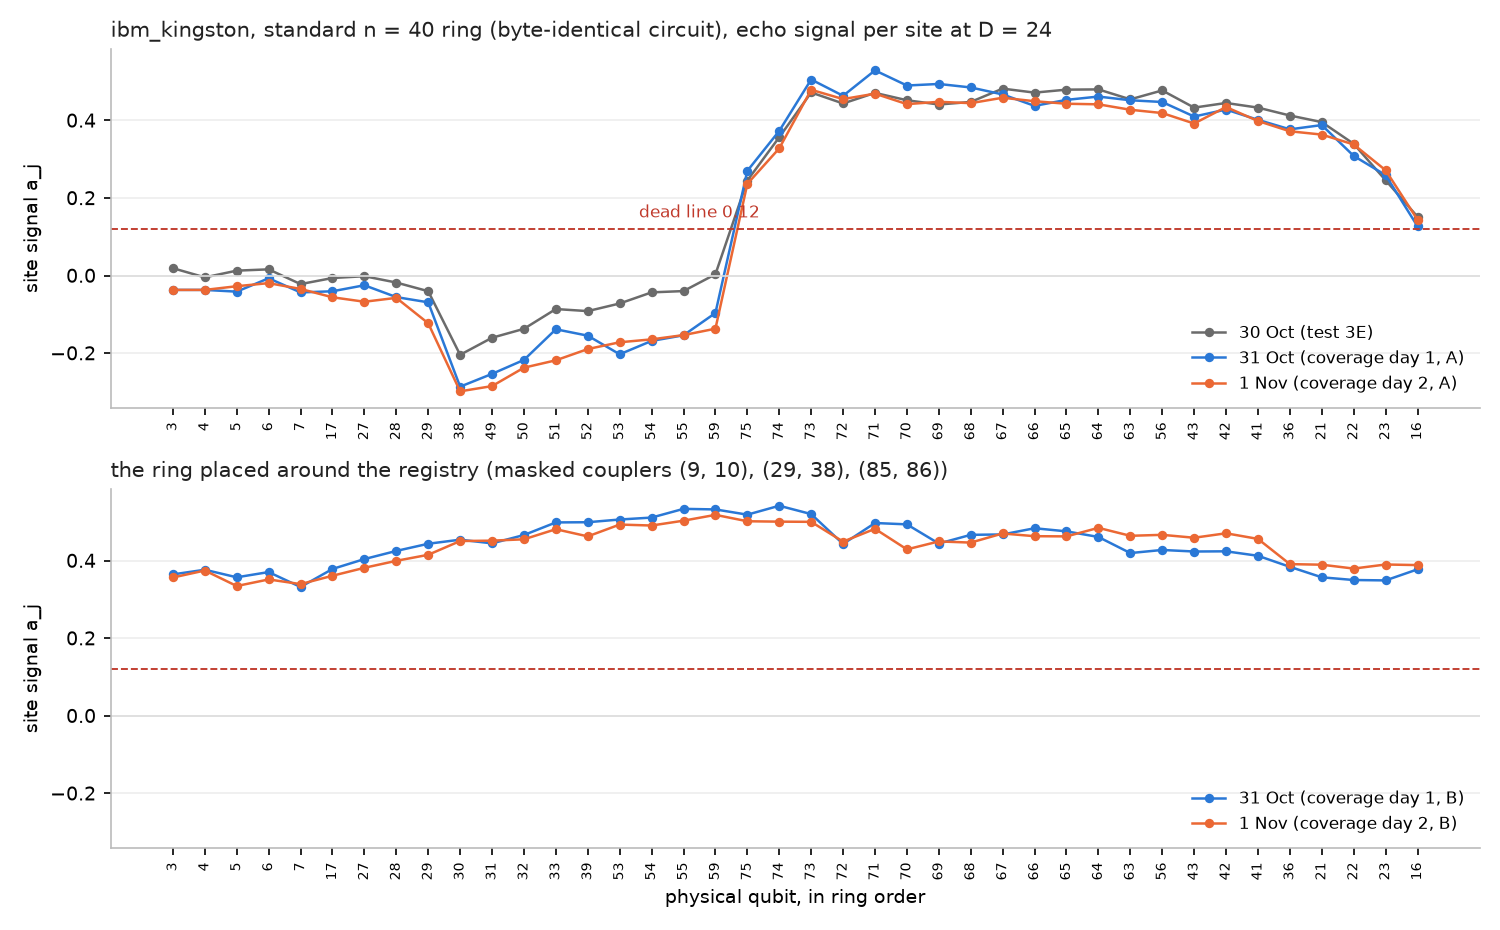
\includegraphics[width=0.93\textwidth]{figures/self_check_kingston_n40_sites.png}
  \caption{\texttt{ibm\_kingston}, echo signal per site at $D=24$. Top: the standard 40-qubit ring on three days; the
  same 18 sites sit below the dead line 0.12. Bottom: the ring placed around the list (masked couplers (9,10), (29,38),
  (85,86)); every site is above it.}
  % src: numbers.json fig1; TOQB results/coverage-days-2026-10-31-day1, results/coverage-days-2026-11-01-day2
  \label{fig:sites}
\end{figure}

\section{The method}

psf-os is a user-side layer. It reads only the device's coupling graph and its failed elements, never a quality
number, and decides from its own runs.

\begin{description}
\item[Scan.] One job of 24 circuits runs a mirror echo of depth $D=24$ on the standard rings and reads a signal $a_j$
  per site. A run of three or more sites below 0.12 is \emph{dead}; a site below $\max(0.12,\,0.5\times\text{median})$
  is \emph{weak}.
  % src: psf-os psf_os/plan.py SCAN_JOB (echo, D=24, h=0.6, 1000 shots); scan thresholds as declared (Paper 6 sec. 3)
\item[Registry.] Each dead run becomes a path entry. A path is \emph{listed} once two jobs agree; an entry expires
  after seven days. A healthy ring that passes a listed path is reported as a contradiction (the entry stays). A weak
  run is kept as a gray mark, avoided on its own day only and never carried over.
  % src: psf-os psf_os/registry.py (entries(): LISTED / CANDIDATE / EXPIRED, contradictions; add_gray(): valid on `day` only)
\item[Avoid.] The allocator masks the middle coupler of each listed path and places the ring by the same fixed rule
  (no search, no seed choice, no selection by simulation). Avoiding is the default.
\item[Sentinel.] The user's job carries four extra echo circuits on the same ring. The result comes back with a
  verdict, CLEAN, WEAK or DEAD, and the sites concerned.
\item[Repair (narrow).] A local frame flip can lift a dead block, but only for mirror-type circuits (Section 4).
\end{description}

Jobs are submitted through the TOQB test bench with ``stay'': a job is never moved to another device. The same build
gives byte-identical compiled circuits (fixed names, recorded SHA-256), so a run can be checked against its manifest.
The time model is $0.036$\,s per circuit $+\;0.00027$\,s per shot $+\;3$\,s per job: about 10\,s for the scan
(9\,s billed in our runs) and about 6.7\,s for an 8-circuit job with its sentinel at 1,000 shots.
% src: psf-os psf_os/job.py qpu_seconds_model; 24*0.036 + 24000*0.00027 + 3 = 10.3 s; 12*0.036 + 12000*0.00027 + 3 = 6.7 s
% src: TOQB results/coverage-days-2026-10-31-day1/README.md (job A, 24 circuits, 9 s billed);
%      results/two-devices-2026-11-01/README.md (scan jobs 9 s; avoid jobs 6 s and 7 s)

\section{Device results}

\textbf{Width.} Every test below was declared before its run (SHA-256 and CET time fixed before the fetch).

\begin{figure}[h]
  \centering
  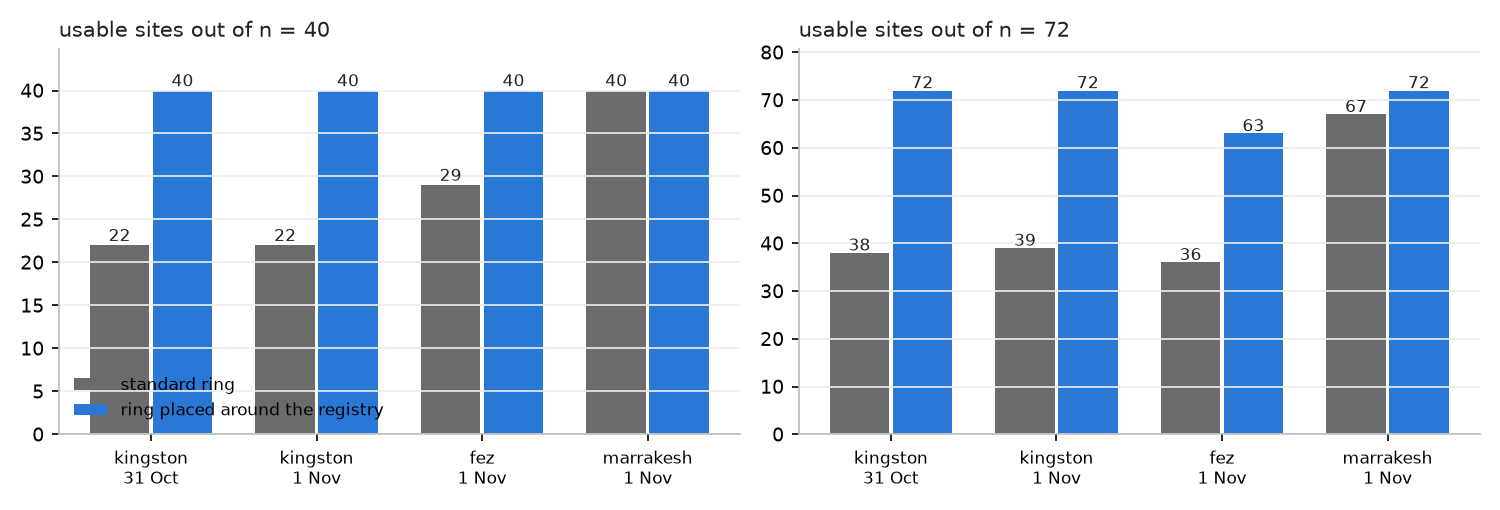
\includegraphics[width=\textwidth]{figures/self_check_width.png}
  \caption{Usable sites (no dead run) on the standard ring and on the ring placed around the list.}
  % src: numbers.json width.*; TOQB results/coverage-days-2026-10-31-day1/coverage.json,
  %      results/coverage-days-2026-11-01-day2/coverage.json, results/two-devices-2026-11-01/{fez,marrakesh}/avoid/coverage.json
  \label{fig:width}
\end{figure}

\begin{table}[h]
\centering\small
\begin{tabular}{lcccc}
\toprule
 & \multicolumn{2}{c}{40-qubit ring} & \multicolumn{2}{c}{72-qubit ring}\\
device, day & usable sites & mean $a_j$ on usable sites & usable sites & mean $a_j$ on usable sites\\
\midrule
kingston, 31 Oct  & 22 $\to$ 40 & 0.41 $\to$ 0.44 & 38 $\to$ 72 & 0.38 $\to$ 0.35\\
kingston, 1 Nov   & 22 $\to$ 40 & 0.39 $\to$ 0.44 & 39 $\to$ 72 & 0.38 $\to$ 0.42\\
kingston, 2 Nov   & 22 $\to$ 40 & 0.41 $\to$ 0.43 & 54 $\to$ 72 & 0.32 $\to$ 0.41\\
fez, 1 Nov        & 29 $\to$ 40 & 0.16 $\to$ 0.20 & 36 $\to$ 63 & 0.27 $\to$ 0.22\\
marrakesh, 1 Nov  & 40 $\to$ 40 & 0.27 $\to$ 0.24 & 67 $\to$ 72 & 0.23 $\to$ 0.26\\
\bottomrule
\end{tabular}
% src: numbers.json width.<device day n>.standard/avoiding/mean_usable (each checked against the TOQB coverage.json)
\caption{Standard ring $\to$ ring placed around the list. The headline is the width; the signal on sites that were
already usable moved little, and fell in three of the ten rows.}
\label{tab:width}
\end{table}

The headline is ``usable sites 22 $\to$ 40''. The essential number is in the second column: on the sites that were
already usable the mean signal moved from 0.41 to 0.44 on kingston, and in three rows it fell. The gain is in how much
of the device can carry a computation, not a better signal everywhere. On fez the placed 72-qubit ring still had nine
unusable sites.

\textbf{A forward computation.} On \texttt{ibm\_marrakesh}, 72 qubits, 12 layers of a computation with a known answer
(not a mirror), on a day when nothing was dead on the standard ring: mean site signal 0.776 on the standard ring and
0.816 on the ring placed around the list ($+0.040\pm0.002$; at 24 layers $+0.052\pm0.002$). The headline is ``per-bit
right 88.8\,\% $\to$ 90.8\,\%''. The essential numbers: all of the gain sits in the ten qubits the placed ring
replaced (0.615 $\to$ 0.866); on the 62 shared qubits the two rings read the same (0.802 against 0.808). The listed
path was weak that day, not dead, so the gain is accuracy, not width.
% src: numbers.json m3b.D12 mean_standard 0.7763, mean_avoid 0.8162, per_bit (0.8881, 0.9081), swapped_mean (0.6148, 0.8663),
%      common_mean (0.8023, 0.8081), n_common 62; m3b.D24 (0.6425, 0.6943)
% src: TOQB results/qca-m3b-2026-11-01/score_S.json, score_V.json (mean_se 0.00114 and 0.00106; combined 0.0016)

\section{Limits}

\begin{itemize}
\item Three devices over three days; one family of circuits (rings placed by one fixed rule, mirror echoes and one
  forward computation). Nothing here is a statement about other circuit families.
\item A first forward test on \texttt{ibm\_kingston} used 40 layers, beyond the readable depth of either ring (0.009
  and 0.020, under the declared floor 0.05). It is reported as INCONCLUSIVE; the design error is ours.
  % src: TOQB results/qca-m3-2026-11-01/README.md; Paper 6 draft sec. 4
\item The frame-flip repair lifted kingston's dead block at 12 layers (block signal 0.27 $\to$ 0.56) but only to about
  0.13 at 24 layers, and it applies only to mirror-type circuits.
  % src: numbers.json repair "31 Oct D12 off" block 0.270, "31 Oct D12 flip at 27, 29" 0.555, "31 Oct D24 flip at 27, 29" 0.129
\item The listed defects are paths. We do not claim their cause. Some dead runs recur at the same ring positions on
  several chips with the same circuit, so part of what a scan sees may depend on the position in the circuit.
  % src: TOQB results/defect-list-replay-2026-10-31/README.md ("n = 72, positions 57-64 on all three devices")
\item The sentinel (M6) is a prototype checked in simulation; it has not yet run on a device.
\end{itemize}

\section{How to try it}

\textbf{Five minutes, no IBM account.} \texttt{POC/quickstart\_os.py} plants a two-qubit depolarizing error
($p=0.15$) on two couplers of IBM's FakeFez in an Aer simulation, scans twice, lists the planted paths, and solves two
practice problems with exact answers on the standard ring and on the placed ring. It prints on its first and last line
that it is a simulation with planted defects, not a device result. One run on a 2-core machine took 92\,s: listed
paths [14,15,19,35] and [74,75,59,55]; cluster-state parity ($n=40$) 0.920 $\to$ 1.000 with sentinel CLEAN; a random
Clifford circuit read through its stabilizers ($n=40$) 0.980 $\to$ 1.000.
% src: quickstart run log (2 Nov 2026), summary.json

\textbf{On a device.} \texttt{psf-os fetch} $\to$ \texttt{psf-os plan} (a scan job first when there is no scan of the
day) $\to$ TOQB \texttt{s2rc\_device submit} (stay) $\to$ \texttt{psf-os scan-ingest} $\to$ \texttt{psf-os plan}
again (placed ring with sentinel) $\to$ \texttt{psf-os result} (score and verdict).

\textbf{Evaluation.} The request form, the mutual NDA template and the report template for psf-os are in
\texttt{POC/}. The test is fixed in writing before anything runs; the report gives the standard and the self-checked
placement side by side.

\textbf{Records.} Paper 5, \emph{Readable Depth Without the Calibration Map}
(\href{https://doi.org/10.5281/zenodo.23827536}{doi:10.5281/zenodo.23827536}); Paper 4
(\href{https://doi.org/10.5281/zenodo.23826764}{doi:10.5281/zenodo.23826764}); Paper 3
(\href{https://doi.org/10.5281/zenodo.23826596}{doi:10.5281/zenodo.23826596}); Paper 6
(\href{https://doi.org/10.5281/zenodo.23883938}{doi:10.5281/zenodo.23883938}) collects the results above. psf-os: \url{https://github.com/TN-Holdings-LLC/psf-os} (pre-release, AGPL-3.0).

\end{document}
